%pb
\documentclass[../../main/main.tex]{subfiles}

\begin{document}


%%%%%%%%%%%%%%%%%%%%% Chapter Patrol Base Operations %%%%%%%%%%%%%%%
\chapter{Patrol Base Operations}\label{chp:pb}
   %%%%%%%%%%%%%%%%%%%% Section Motivation %%%%%%%%%%%%%%%%%%%%%%
\section{Motivation}
The aim of this master thesis is to demonstrate proof of applicability (or failure) of \glsentryshort{csbd} to non-automated, human centered systems.  Military operations are a great example because safety and security are critical to mission success.  The patrol base operations are an excellent example of non-automated, human-centered military operations.

   %%%%%%%%%%%%%%%%%%% Section Ranger Handbook Description %%%%%%%%%%%%%
\section{Patrol Base Operations}
Patrol base operations are described in the United States Army Ranger Handbook \cite{rangermanual} in chapter 7 (2017 edition).  The mission activity specification for the patrol base operations are shown in table \ref{pbtab}

\parskip=8pt
\begin{table}[h!]
\begin{center}
\begin{tabular}{ | m{3.3em} | m{3.8cm}| m{9cm} | } 
\hline
\multicolumn{3}{|c|}{Patrol Base Operations: Mission Activity Specification} \\
\hline \hline
Purpose & A system to & establish a security perimeter when a squad or platoon halts for an extended period of time \\ 
\hline
Method & by means of  & planning, reconnaissance, security, control, and common sense  \\ 
\hline
Goal & in order to & 
\begin{itemize}
\item avoid detection
\item hide a unit during a long, detailed reconnaissance
\item perform maintenance on weapons, equipment, eat, and rest
\item plan and issue orders
\item reorganize after infiltrating an enemy area
\item establish a base from which to execute several consecutive or concurrent operations
\end{itemize}

 \\ 
\hline
\end{tabular}
\end{center}
\caption{Mission Activity Specification for Patrol Base Operations.  Adapted from the U.S. Army Ranger Handbook 2017 \cite{rangermanual}.}
\label{pbtab}
\end{table}
\parskip=18pt

This master thesis applies properties of complete mediation to a model of these patrol base operations.

   %%%%%%%%%%%%%%%%%%% Section Describing The Patrol Base Operations %%%%%%%%
\section{Modeling the Patrol Base Operations from the Ranger Handbook}\label{sec:modelingpb}
\glsresetall[\acronymtype]

Modeling a system requires the knowledge of an expert on the system.  This is necessary because only someone who is familiar with the system, especially with regards to security, can detail its nuances.  For this reason, a subject matter expert from the United States Army (Jesse Nathaniel Hall) is employed to develop a model of the patrol base operations. 

The model of the patrol base operations needs to be amiable to complete mediation and verification using an access-control logic (section \ref{sec:acl}).  This is necessary to prove security properties of the patrol base operations.  To do this, the patrol base operations are abstracted from the Ranger Manual and modeled in Visio\footnote{This work began as a collaboration between Jesse Nathaniel Hall and the author.  Once the hierarchy of secure state machines was decided upon, the abstraction of the Ranger Handbook was done by Jesse Nathaniel Hall with only structural consultation with the author.  Concurrently, the author focused on proving the properties of complete mediation in the ACL using HOL.  Thus, there was a great deal of separation of work.  Jesse's work is described here because it is necessary to put the entire system into context for this master thesis.  This means that Jesse's work provided the model of the system for which the principle of complete mediation was proved, verified and documented.}.  The result of doing this is a hierarchy of secure state machines (\glsentryshortpl{ssm}). (\glsentryshortpl{ssm} are described in section \ref{sec:ssm}.)  

\section{Overview of The Hierarchy of Secure State Machines}\label{sec:overview}

Each level of the hierarchy of \glsentryshortpl{ssm} represents a level of abstraction of the patrol base operations. The most abstract level of the hierarchy is the top level \glsentryshort{ssm}.  A diagram of this most abstract level is shown in figure \ref{pbtoplevel}.

\begin{figure}[h]
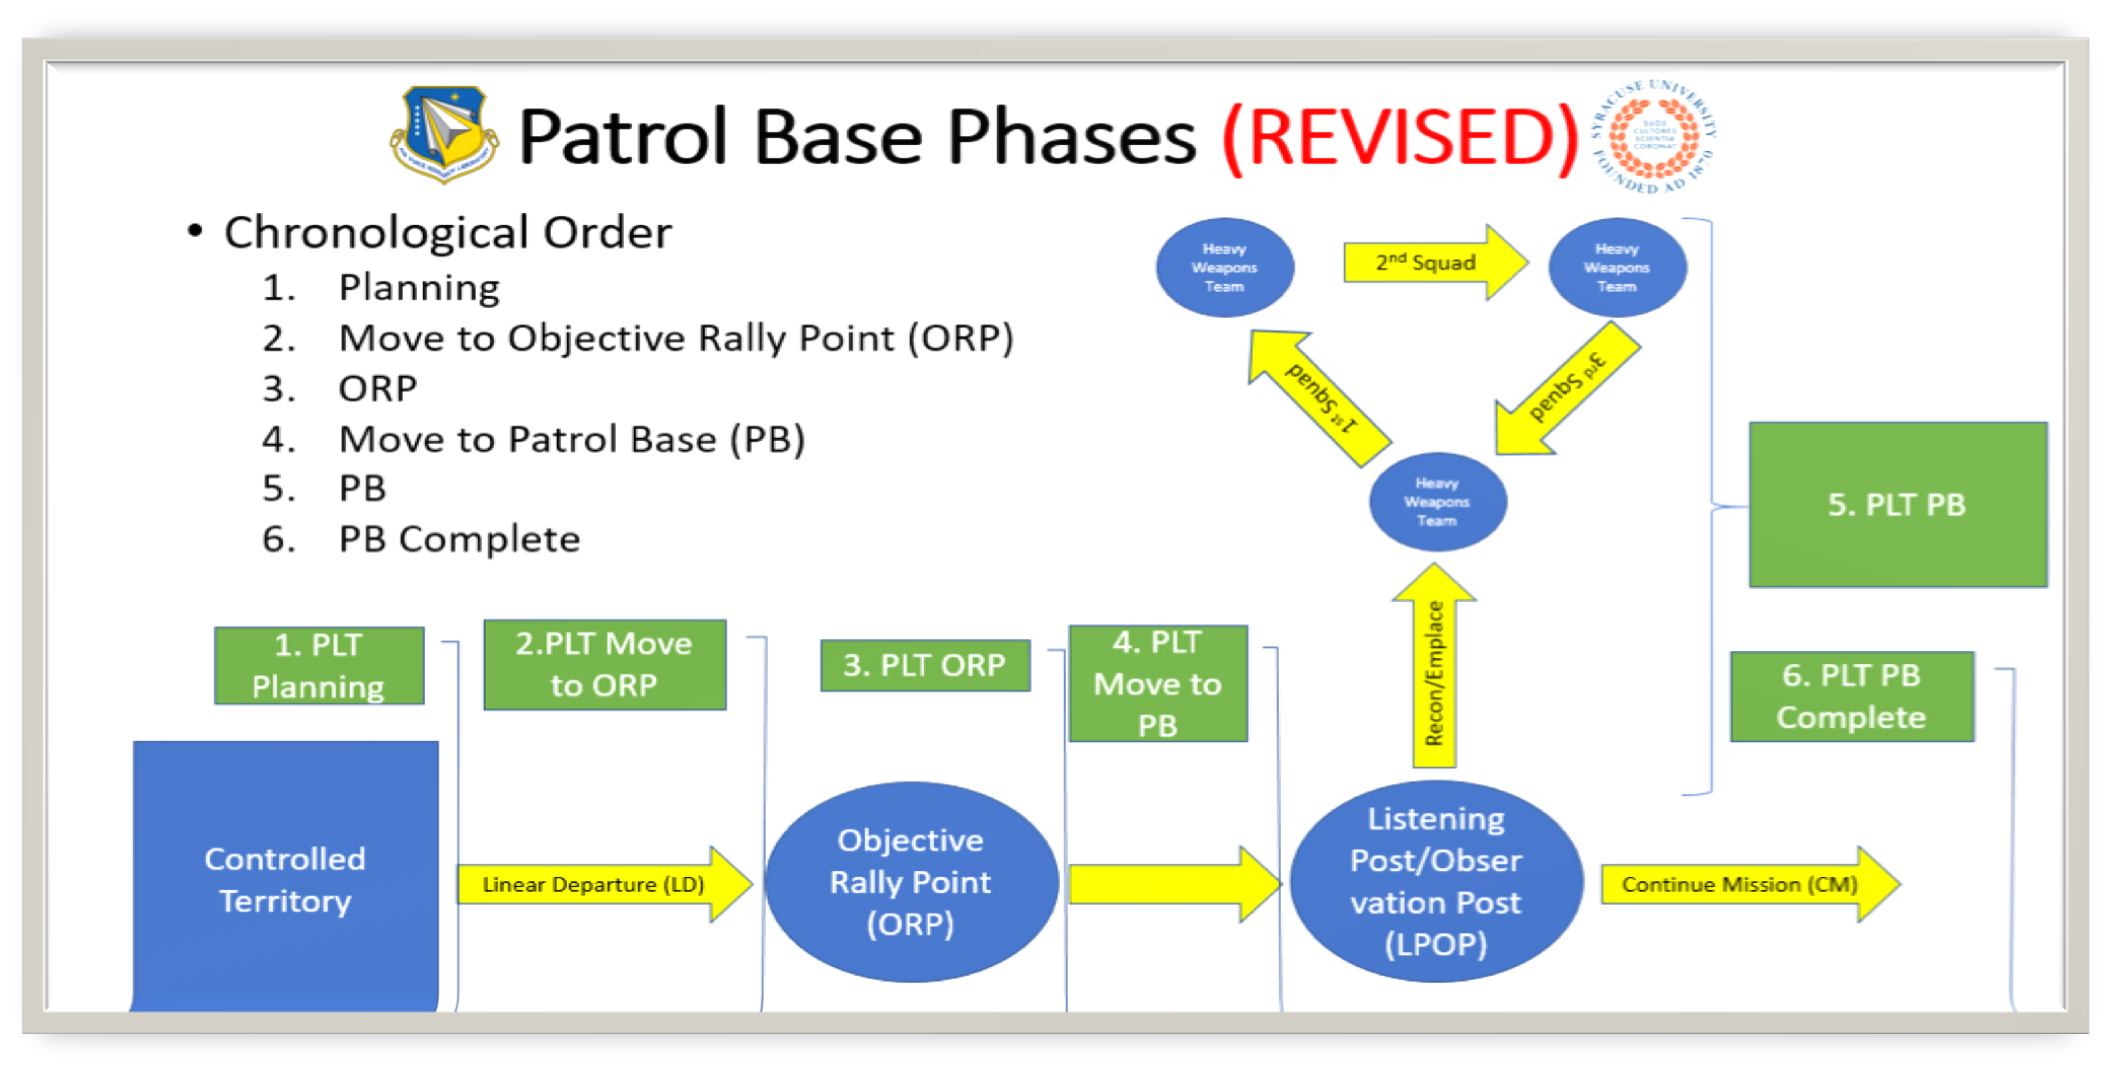
\includegraphics[width=\textwidth]{../figures/pbtoplevel}
\caption{\label{pbtoplevel}A diagram of the most abstract level in the hierarchy of secure state machines.  Image generated by Jesse Nathaniel as part of the research involved in this master thesis.  Shall I get his permission?}
\end{figure}

The diagram describes a chronological order of abstract phases (modeled as states) of the patrol base operations.  The operations begin with the planning phase (1).  Next, they move to the objective rally point (\glsentryshort{orp}) (2). At the \glsentryshort{orp}, operations commence (3).  When these are complete, the patrol base operations move to the actual patrol base (4).  At the patrol base, operations proceed (5).  Finally, the patrol base operations are complete (6).  These are the six states in the top level \glsentryshort{ssm}.


The next level of abstraction in the hierarchy of \glsentryshortpl{ssm} represents a horizontal slice through the patrol base operations.  This is the second level of the hierarchical description of the patrol base operations. It is referred to as the sub level.  In this documentation, \glsentryshortpl{ssm} at this level are referred to as the sub-level, sublevel, or subLevel \glsentryshortpl{ssm}. This slice describes the patrol base operations at a lower level of abstraction.  It expands each of the states in the top level (except for the last state PB Complete).  For example, the planning phase (1) in figure \ref{pbtoplevel} is expanded into an \glsentryshort{ssm} of its own.  This is called ssmPlanPB.  It consists of several states (see section \ref{sssec:ssmPlanPB}) which detail activities conducted during the planning phase of the patrol base operations.  Each state in the top level (except for PB Complete) has it's own \glsentryshort{ssm} (see the next section).

At yet another lower level of abstraction is the sub-sub (3rd) level.  In this documentation, \glsentryshortpl{ssm} at this level are referred to as the sub-sub-level, subsublevel, or subsubLevel \glsentryshortpl{ssm}.  This level expands upon the states in the sub level (one level above) in the same manner that the sub level expands upon the states in the top level \glsentryshort{ssm}.  In this manner, each level is a lower level of abstraction than the level above it. 

A vertical slice through the diagram is also modeled.  This slice models the patrol base operations from the top level down to the most detailed level (level 8).  This vertical slice consists of a series of \glsentryshortpl{ssm}.  Each \glsentryshort{ssm} expands upon only one state in the level above it.  This differs from the horizontal slice which expands upon all states in the level above it.  Expanding upon only one state focuses on a vertical slice through all 8 states of the hierarchy of \glsentryshortpl{ssm}.

The vertical slice begins at the top level \glsentryshort{ssm}.  Next, it expands upon one state at this level, the \textit{move to ORP} state (2).  This results in a sub level \glsentryshort{ssm} named ssmMoveToORP.  The vertical slice progresses in this manner, by expanding one state at each level into a new \glsentryshort{ssm}.  From ssmMoveToORP, the state \textit{secure halt} is expanded to ssmSecureHalt.  From within this \glsentryshort{ssm}, the state \textit{ORP Recon} is expanded into ssmORPRecon.  From within this \glsentryshort{ssm}, the state \textit{Move to ORP 4L} (fourth level move to ORP state) is expanded into ssmMoveToORP4L.  Finally, from within this \glsentryshort{ssm}, the state \textit{Form RT} is expanded into ssmFormRT.

The vertical slice spans the all eight levels.  However, not all levels are represented with an \glsentryshort{ssm}.  The last \glsentryshort{ssm} in the vertical slice, ssmFormRT, is actually at the 5th level of the hierarchy.  This \glsentryshort{ssm}, consists of three states.  These three states reside at the 7th level because ssmFormRT does not have states at the 6th level (it skips the 6th level).  Furthermore, the 7th level states are not expanded into an \glsentryshort{ssm} because each of these 7th level states expand into only one state at the 8th level.  

In addition to the horizontal and vertical slices, an escape level is also modeled.  Actions in the escape level are reachable from any phase of the patrol base operations.  These actions are the unacceptable circumstances that require the patrol base operations to abort.  For example, if the patrol base contacts the enemy in any phase of the operations, then the command \textit{react to combat} is issued.  The patrol base operations are subsequently aborted.  

Excluding the escape level, there are eight levels of the hierarchy of \glsentryshortpl{ssm}.

Note that, the purpose of this master thesis is only to demonstrate that the properties of complete mediation could be applied and verified on a non-automated, human-centered systems. Thus, it is sufficient to demonstrate this on a horizontal and vertical slice of the patrol base operations\footnote{Otherwise, the author would not graduate because the patrol base operations are huge.  }.  

   %%%%%%%%%%%%%%%%%%% Section Hierarchy of Secure State Machines %%%%%%%%%%
\section{Hierarchy of Secure State Machines}
\begin{figure}[h]
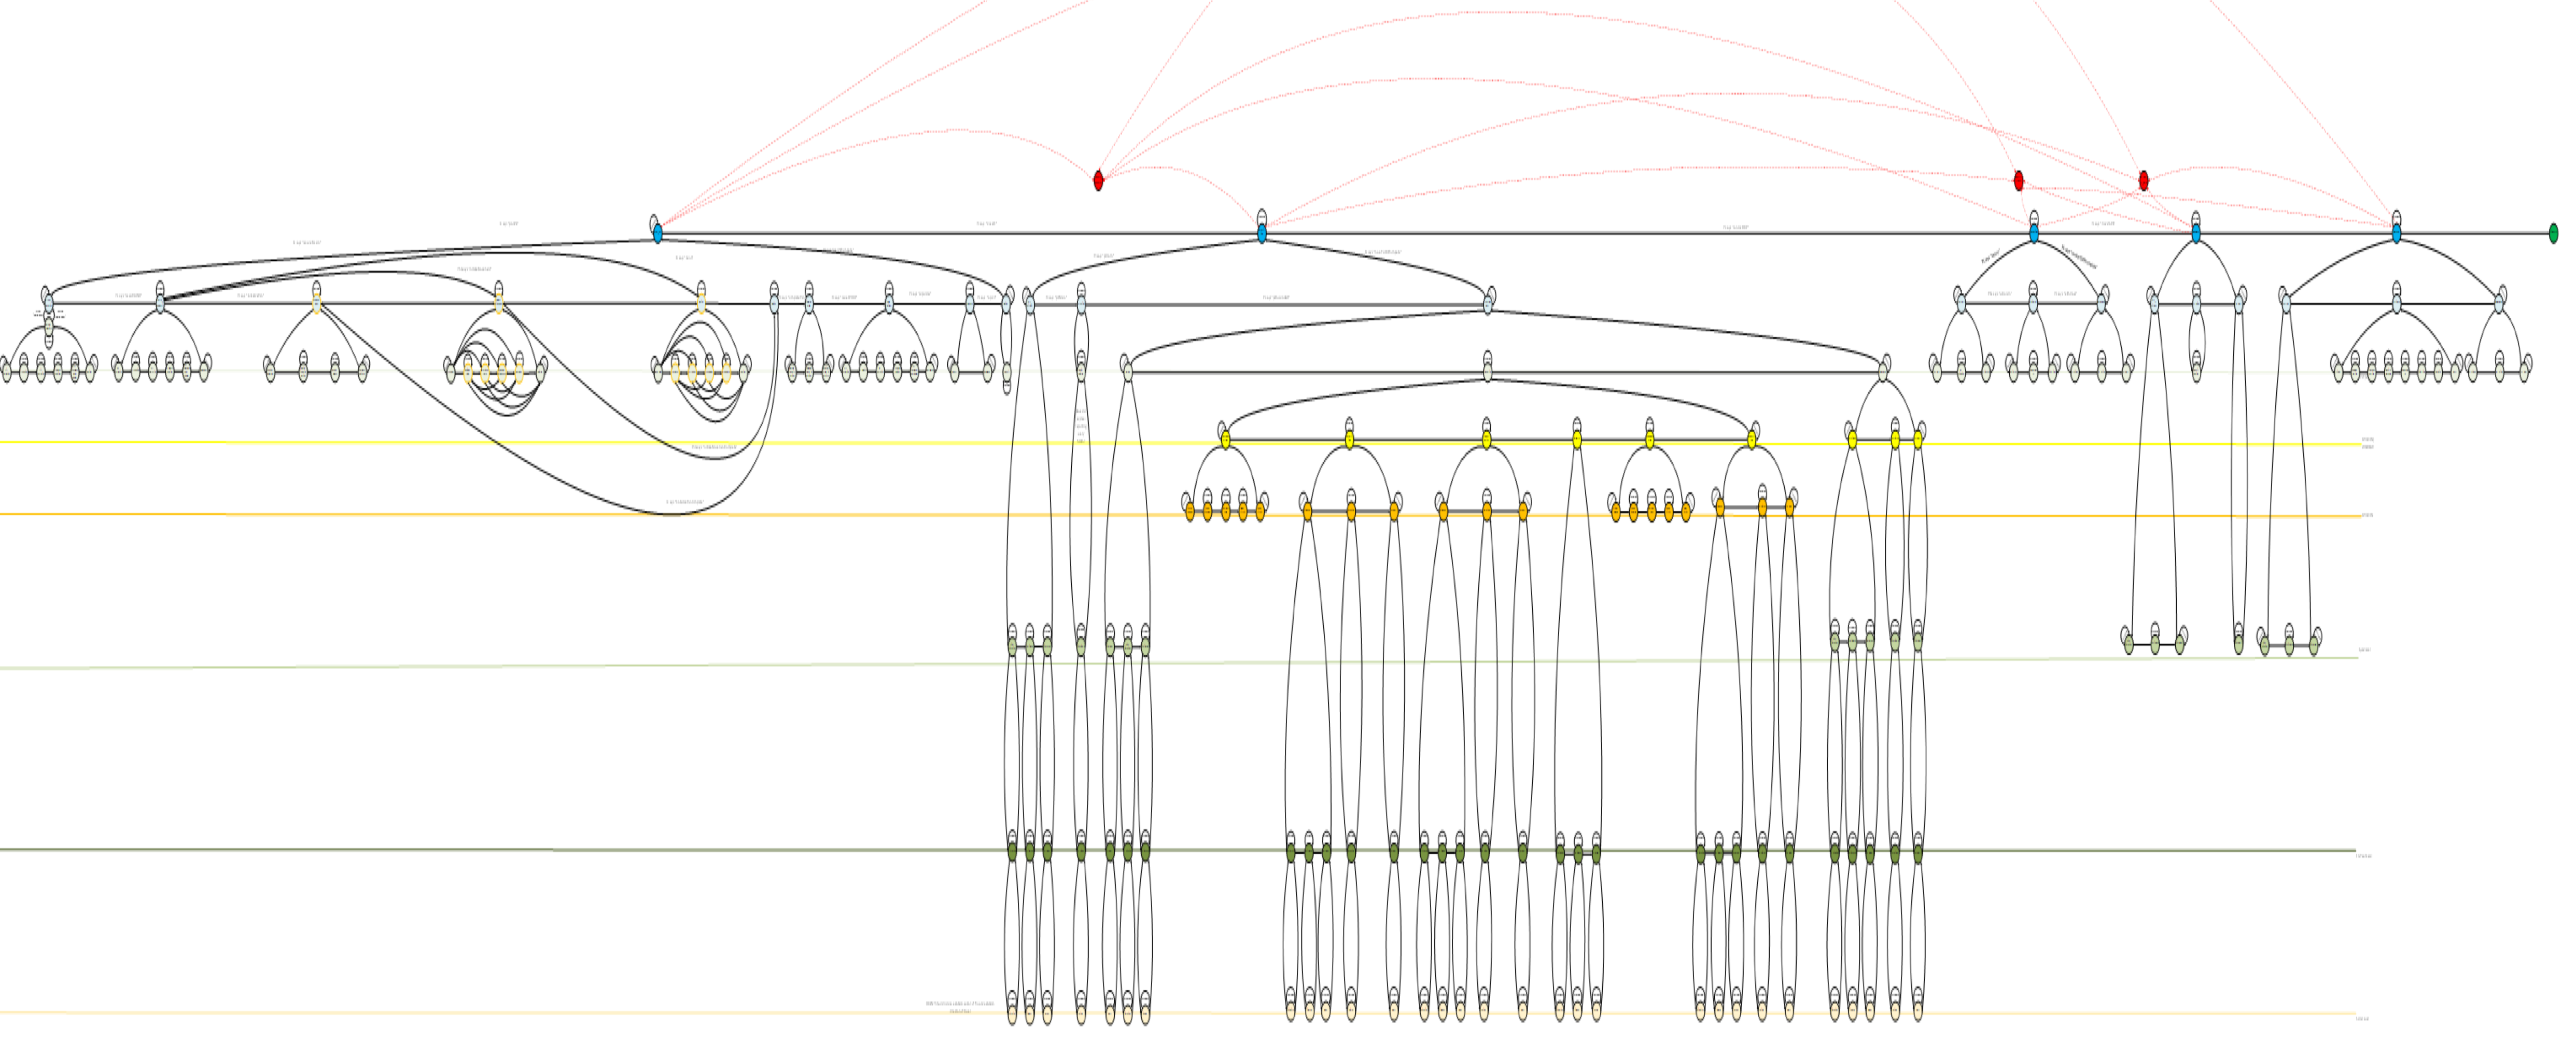
\includegraphics[width=\textwidth]{../figures/overalldiagramsquashed}
\caption{\label{overalldiagramsquashed}Diagrammatic description of patrol base operations as a hierarchy of secure state machines.  (Generated by Jesse Nathaniel Hall.)}
\end{figure}

          %%%%%%%%%%%%%%%% Subsection Diagrammatic Description %%%%%%%%%%%%%%
\subsection{Diagrammatic Description in Visio}\label{ssec:overalldiagram}
The enormity of the hierarchy of \glsentryshortpl{ssm} is evident in figure \ref{overalldiagramsquashed}.  This is a squashed version of the Visio diagram for the hierarchy of \glsentryshortpl{ssm}. The diagram is included as a Visio file with the files for this project (LaTeX/figures/diagram.vis).  



The straight, colored lines that span the diagram in figure \ref{overalldiagramsquashed} delineate levels of the hierarchy of \glsentryshortpl{ssm}.  The top lines are obscured by the size of this squashed version of the diagram.  The most visible bright yellow line delineates the sub-sub-sub (4th) level of the hierarchy, for example.

This is actually only a partial represenation of the patrol base operations.  The middle section that extends to the bottom of the diagram represents a vertical slice through the model of the patrol base operations.  For most sections, the diagram does not extend below to the yellow horizontal line spanning the diagram.  


The small, colored dots in figure \ref{overalldiagramsquashed} represent states (phases) of the patrol base operations.  The red dots are an exception.  The labels for these states are not readable in this diagram.  The dots are color coded.  The colors correspond to the level of those states.  For example, the dots at the top level (level below the red dots) are all dark blue.  

In figure \ref{overalldiagramsquashed}, the red dots at the top of the diagram represent the escape level \glsentryshort{ssm}.  But, they do not represent states in the \glsentryshort{ssm}.  This is because the escape level  \glsentryshort{ssm} is accessible by all phases of the patrol base operations.  This means that if can not be ascribed to any one level of the hierarchy. 


The dots representing states are connected to each other by lines.  These lines represent allowable transitions from one state to another.  The escape level is again an exception.  If no line connects one state to another then no transition is allowed.  

The red dots representing the escape level \glsentryshort{ssm} are best thought of as multiple copies of a floating \glsentryshort{ssm}.  The escape level \glsentryshort{ssm} acts as a sub-\glsentryshort{ssm} for all \glsentryshortpl{ssm} in the hierarchy.  During patrol base operations, abortion of the patrol base operations can occur at any action from any state at any level.  This means that any state at any level can be terminated by the escape level \glsentryshort{ssm}.  Drawing lines from all states to the escape level \glsentryshort{ssm} and drawing really long lines clutters the diagram.  Therefore, only lines at the top level are drawn and the red dots are duplicated.

 The lines in the diagram are annotated by \glsentryshort{ssm} requests.  (Annotations are visible in the original Visio diagram, but not in this squashed version.)  For example, a line connecting the top level state PLAN_PB is annotated with the request \textit{PlatoonLeader says crossLD}.  crossLD is an abbreviation for "cross the line of discrimination" and it is the command to transition to the MOVE_TO_ORP state.    Lines are not annotated beyond the sub level.

Details of each level follow in the next section.

\subsection{Descriptions of Individual Modules}
Each module is described diagrammatically in the following sections.  They all follow a similar pattern.  The general pattern is discussed in this section.  Exceptions are discussed along with the diagrammatic descriptions for each individual module. (Note also that "module" and "SSM" are used interchangeably in the following sections.)

\paragraph*{Flow}
Each module follows a sequential pattern.  It starts at one state and then flows sequentially to the end of the module. Each module has a set of principals who are authorized on some set of transitions (or commands).  Each module has its own security policy that dictates the conditions under which transition requests are granted.  

\paragraph*{Requests And Security Policies}
Principals make requests to transition from one state to another.  Requests are of the form \textit{Principal says command}.  

Transitions at one level require confirmation of completion of that state at the lower level.  For example, the PLAN_PB state at the top level is the basis for the less abstract ssmPlanPB secure state machine one level below it.  Before the top level can transition from the PLAN_PB state to the MOVE_TO_ORP state, ssmPlanPB must be in the COMPLETE state.  

But, encapsulation requires that each module be isolated from the other.  To accommodate this, an OMNI level principal communicates when a sub level is complete. Thus, transitions from one state to another require a statement from OMNI and a request from an authorized authority.  An example is \textit{OMNI says ssmPlanPBComplete} and \textit{PlatoonLeader says crossLD}.

The security policy for each module has a policy for OMNI and a policy for all authorized principals.  For OMNI, the security policy contains the clause \textit{OMNI controls omniCommands}.  In the example above, the command ssmPlanPBComplete is defined as an omniCommand.  For everyone else, the security policy has clauses of the form \textit{ssmPlanPBComplete impf (PlatoonLeader controls crossLD)}.  This is sufficient to prove complete mediation for transitions.


\paragraph*{Diagrammatic Description}
The colors of the states in the diagrams correspond to their colors in the overall squished diagram shown in figure \ref{overalldiagramsquashed}.  

All lines represent allowable transitions with an arrow indicating the direction of the transition.  Each line is annotated with the appropriate \glsentryshort{acl} request (or command).  The last line in each module is an exception.  It connects the COMPLETE state to the initial state.  This line is not annotated.  It is not an actual transition but an indictor that the completion of this lower-level \glsentryshort{ssm} links to the higher-level \glsentryshort{ssm}.  It is implemented in the \glsentryshort{ssm} above it as a signal from the OMNI level\footnote{OMNI is all knowing.} that the lower-level \glsentryshort{ssm} is complete\footnote{Note, it is possible that the output for the transition to the COMPLETE state is \textit{OMNI says ssmPlanPBComplete}.  This may or may not have been implemented in the \glsentryshort{hol} proofs at the time this master thesis was complete.}. 

\paragraph*{Naming conventions}
What follows are the naming conventions for the diagrams.  The also apply to the \glsentryshort{hol} implementation of the \glsentryshortpl{ssm}.
\begin{description}
\item[state: ] all capital letters with underscores representing spaces.  Examples include: MOVE_TO_ORP, PLAN_PB, etc.
\item[commands (or requests):] first letter is lower case.  The remaining letters toggle with a capital letter for each new word.  Examples include: moveToORP,  receiveMission, etc.  Furthermore, all commands take the name of the next state. For example, the transition from the state MOVE_TO_PB to CONDUCT_PB is conductPB.  The transition from the state COMPLETE_PLAN to ISSUE_OPORD is issueOPORD.  The only exception is the transition from the top level state PLAN_PB to the next state MOVE_TO_ORP.  The command for this transition is crossLD and not moveToORP.
\item[principals:] all begin with a capital letter then follow the convention for commands (or requests).  Examples include: PlatoonLeader, PlatoonSergeant, etc.
\item [\glsentryshort{acl} transition requests:] all are of the form \textit{Principal says command}.  Examples include: \textit{PlatoonLeader says moveToORP}, \textit{PlatoonSergreant says actionsIn}, etc.
\end{description}

          %%%%%%%%%%%%%%%% Subsection OMNI-Level %%%%%%%%%%%%%%%%%%%%%
\subsection{OMNI-Level}\label{ssec:omnilevel}
The OMNI level is not represented in the Visio diagram.  It is not really a level.  More specifically, the OMNI level represents an imaginary all-knowing entity.  The main purpose of this entity is to relay messages from one \glsentryshort{ssm} to another.  This allows for greater encapsulation of the modules. 

In all \glsentryshortpl{ssm}, OMNI is a principal who has authority over OMNI level commands.  These commands communicate the completion of a lower-level \glsentryshort{ssm}.  For example, at the top level, before the Platoon Leader can transition from the PLAN_PB state to the MOVE_TO_ORP state, he must receive the command \textit{OMNI says ssmPlanPBComplete}.  The top level security policy contains the clause \textit{OMNI controls ssmPlanPBComplete}.  The \textit{Controls} rule discussed in section \ref{ssec:inferencerules} then allows the Platoon Leader to conclude that the lower-level \glsentryshort{smm} is complete.  
\clearpage


%OMNI serves as an integrating principal.  OMNI was created to accommodate encapsulation of all the secure state machines.  OMNI "knows" when one secure state machine is complete and then conveys that information to other secure state machines as needed.  For example, In the top level \glsentryshort{ssm}, transition from the PLAN_PB state to the MOVE_TO_ORP state requires completion of the ssmPlanPB secure state machine.  OMNI knows when this happens and relays that information to the top level \glsentryshort{ssm}.  In this way, the top level knows what is happening at other levels only through OMNI and need not be concerned with the lower level \glsentryshortpl{ssm} otherwise.



          %%%%%%%%%%%%%%%% Subsection Escape %%%%%%%%%%%%%%%%%%%%%%%
\subsection{Escape}\label{ssec:escape}
A diagram of the escape level is shown in figure \ref{escapeDiagram}.  The purpose of the escape level is to model situation wherein the patrol base operations must be aborted.  

\begin{figure}[h!]
\centering
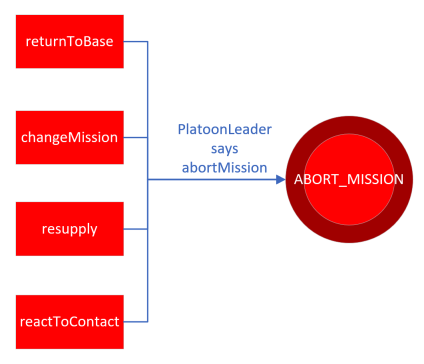
\includegraphics[width=0.45\textwidth]{../figures/escapeDiagram}
\caption{\label{escapeDiagram} Escape level diagram.}
\end{figure}

This is also not really a  level, nor is it an \glsentryshort{ssm}. The square boxes in the diagram represent communication from outside the module.  They represent external signals from the OMNI level.  The only state is the ABORT_MISSION state.  But, one state is not sufficient for an \glsentryshort{ssm}\footnote{This is not necessarily a rule.  But, for the purposes of this master thesis it is a rule.}.

The abortable conditions are \textit{returnToBase}, \textit{changeMission}, \textit{resupply}, and \textit{reactToContact}.  OMNI receives information from somewhere else that one of these conditions is true, for example \textit{returnToBase}.  In response, OMNI submits a request to the escape level:  \textit{OMNI says returnToBase} (etc.).  The security policy for the escape level contains the clause \textit{OMNI controls returnToBase}.  Using the \textit{Controls} rule discussed in section \ref{ssec:inferencerules}, the proposition \textit{returnToBase} must be true.  

Now, the Platoon Leader makes a request to abort the mission: \textit{PlatoonLeader says abortMission}.  Another clause in the security policy is \textit{returnToBase impf PlatoonLeader controls abortMission}.  There is now sufficient information to justify aborting the mission. 
 \clearpage

          %%%%%%%%%%%%%%%% Subsection Top Level %%%%%%%%%%%%%%%%%%%%%%
\subsection{Top Level}\label{ssec:toplevel}
The top level for the hierarchy of \glsentryshortpl{ssm} is shown in figure \ref{ssmPBDiagram}.  This is a linearized version of figure \ref{pbtoplevel}.

\begin{figure}[h!]
\centering
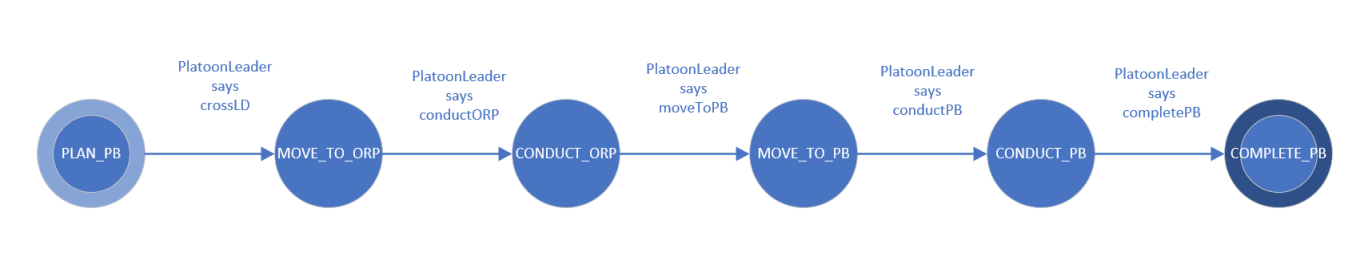
\includegraphics[width=\textwidth]{../figures/ssmPBDiagram}
\caption{\label{ssmPBDiagram} Top level diagram.}
\end{figure}

 The details are discussed along with figure \ref{pbtoplevel}.  The only difference in this diagram is that the state names are all capitalized with underscores substituted for spaces.

 \clearpage

          %%%%%%%%%%%%%%%% Subsection Horizontal Slice %%%%%%%%%%%%%%%%%%%
\subsection{Horizontal Slice}\label{ssec:horizontalslice}
The horizontal slice is an expansion of the states in the top level \glsentryshort{ssm}.  Each state save for the COMPLETE_PB state is expanded into an \glsentryshort{ssm}.  Each of these \glsentryshortpl{ssm} is described in the following sections.

                  %%%%%%%%%%%%% Subsection ssmPlanPB %%%%%%%%%%%%%%%%%%%%%
\subsubsection{ssmPlanPB}\label{sssec:ssmPlanPB}
The top level PLAN_PB state is expanded into the ssmPlanPB \glsentryshort{ssm} and shown in figure \ref{ssmPlanPBDiagram}.

\begin{figure}[h!]
\centering
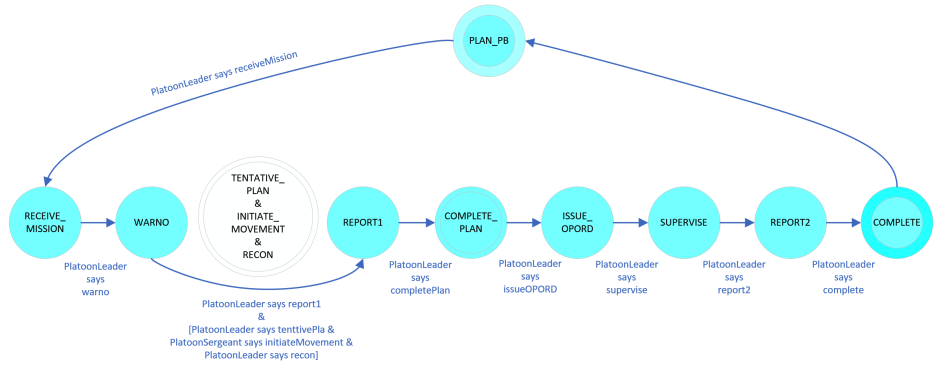
\includegraphics[width=\textwidth]{../figures/ssmPlanPBDiagram}
\caption{\label{ssmPlanPBDiagram} Horizontal slice: PlanPB diagram.}
\end{figure}


ssmPlanPB has two principals: PlatoonLeader and PlatoonSergeant.  Only the PlatoonLeader is authorized to make transitions among states.  

All transitions are sequential.  However, the original module contains three non-sequential states.  These are represented in the diagram as the white circle. These states are TENTATIVE_PLAN, INITIATE_MOVEMENT, and RECON.  To transition from WARNO to REPORT1 requires that all three of these states be completed, but not in any specific order\footnote{The complexities of this \glsentryshort{ssm} lead to a revision of the original parameterized \glsentryshort{ssm} discussed in chapter \ref{chp:ssmmodel} section \ref{sec:sminHOL}.}. 

To solve this problem, the three states are not represented as states.  The completion of these "tasks" is indicated by the following three statements: \textit{PlatoonLeader says tentativePlan}, \textit{PlatoonSergeant says initiateMovement}, and \textit{PlatoonLeader says recon}.  Thus, the transition from WARNO to REPORT1 now requires four statements: \textit{PlatoonLeader says tentativePlan}, \textit{PlatoonSergeant says initiateMovement}, \textit{PlatoonLeader says recon}, \textbf{AND} \textit{PlatoonLeader says report1}. The latter-most statement is the actual request.

To be certain that the transition from WARNO to REPORT1 occurs if and only if these three statements are made, the security policy has an additional clause: \textit{tentativePlan andf initiateMovement andf recon impf PlatoonLeader controls report1}.  In the \glsentryshort{hol} a function extracts \textit{tentativePlan} from \textit{PlatoonLeader says tentativePlan}, and so on for all three statements. The security policy uses this function to verify that all four statements are present in the request to transition.

Note that these three statements are made without authentication and authorization.  It wouldn't be too much effort to add this.  But, these communications can also be thought of as the Platoon Leader receiving these statements directly from the sources.  In this case, the Platoon Leader should recognize himself and his Platoon Sergeant.  The actual implementation for a real world application would need to consider which is most appropriate for the situation.



\clearpage
                  %%%%%%%%%%%%% Subsection ssmMoveToORP %%%%%%%%%%%%%%%%%%%
\subsubsection{ssmMoveToORP}\label{sssec:ssmMoveToORP}
The top level MOVE_TO_ORP state is expanded into the ssmMoveToORP \glsentryshort{ssm} and shown in figure \ref{ssmMoveToORPDiagram}.

\begin{figure}[!h]
\centering
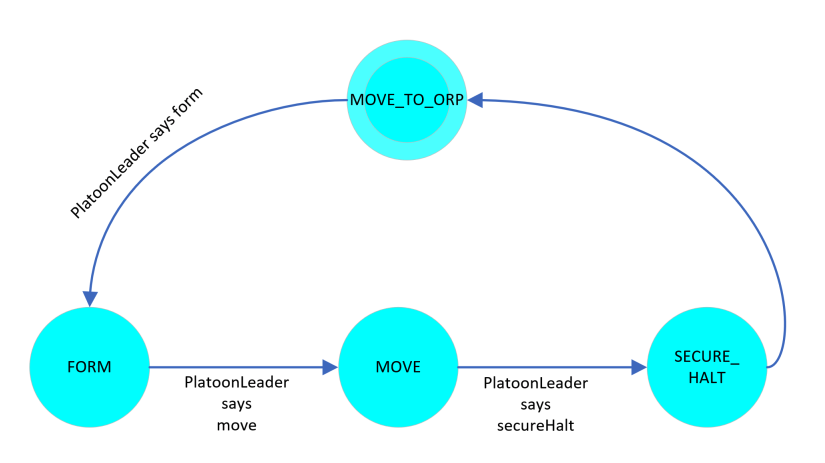
\includegraphics[width=0.8\textwidth]{../figures/ssmMoveToORPDiagram}
\caption{\label{ssmMoveToORPDiagram} Horizontal slice: MoveToORP diagram.}
\end{figure}

ssmMoveToORP is straight forward. There is only one principal authorized to make transitions.  This is the Platoon Leader.  Everything follows sequentially.  
\clearpage

                  %%%%%%%%%%%%% Subsection ssmConductORP %%%%%%%%%%%%%%%%%%
\subsubsection{ssmConductORP}\label{sssec:ssmConductORP}
The top level CONDUCT_ORP state is expanded into the ssmConductORP \glsentryshort{ssm} and shown in figure \ref{ssmConductORPDiagram}.


\begin{figure}[h!]
\centering
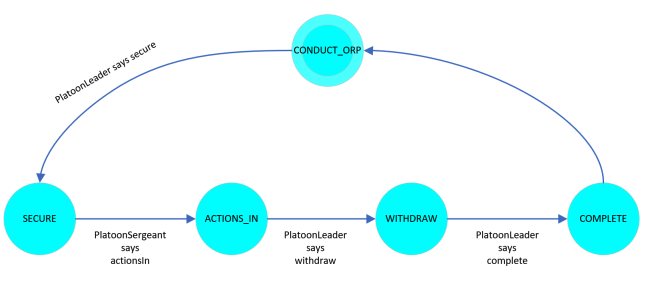
\includegraphics[width=\textwidth]{../figures/ssmConductORPDiagram}
\caption{\label{ssmConductORPDiagram} Horizontal slice: ConductORP diagram.}
\end{figure}

ssmConductORP is straight forward. But, there are two principals. The PlatoonLeader is authorized on all transitions except for the transition from SECURE to ACTIONS_IN.  The PlatoonSergeant is responsible for this transition.  Everything follows sequentially.  

\clearpage

                  %%%%%%%%%%%%% Subsection ssmMoveToPB %%%%%%%%%%%%%%%%%%%
\subsubsection{ssmMoveToPB}\label{sssec:ssmMoveToPB}
The top level MOVE_TO_PB state is expanded into the ssmMoveToPB \glsentryshort{ssm} and shown in figure \ref{ssmMoveToPBDiagram}.

\begin{figure}[h!]
\centering
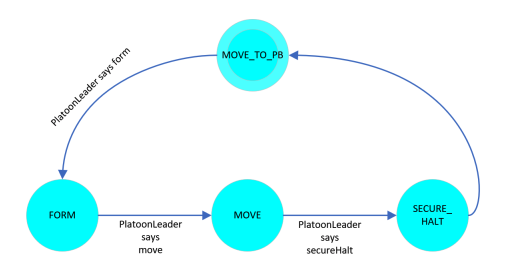
\includegraphics[width=0.8\textwidth]{../figures/ssmMoveToPBDiagram}
\caption{\label{ssmMoveToPBDiagram} Horizontal slice: MoveToPB diagram.}
\end{figure}

ssmMoveToPB is straight forward. There is only one principal authorized to make transitions.  This is the Platoon Leader.  Everything follows sequentially.  
\clearpage
                  %%%%%%%%%%%%% Subsection ssmConductPB %%%%%%%%%%%%%%%%%%%
\subsubsection{ssmConductPB}\label{sssec:ssmConductPB}
The top level CONDUCT_PB state is expanded into the ssmConductPB \glsentryshort{ssm} and shown in figure \ref{ssmConductPBDiagram}.

\begin{figure}[h!]
\centering
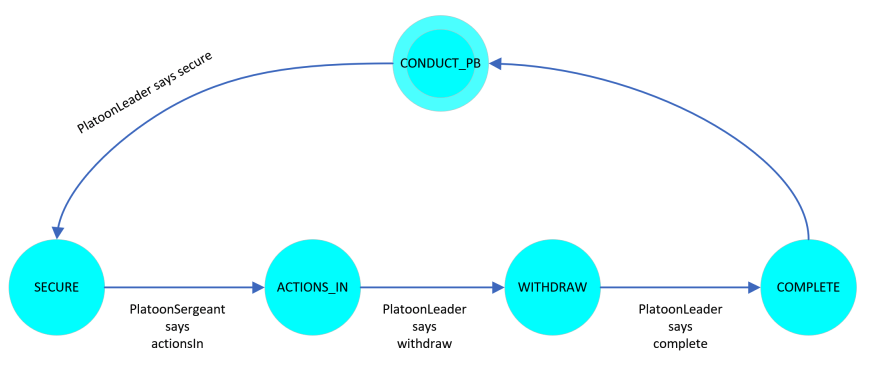
\includegraphics[width=\textwidth]{../figures/ssmConductPBDiagram}
\caption{\label{ssmConductPBDiagram} Horizontal slice: ConductPB diagram.}
\end{figure}

ssmConductPB is straight forward. But, there are two principals. The PlatoonLeader is authorized on all transitions except for the transition from SECURE to ACTIONS_IN.  The PlatoonSergeant is responsible for this transition.  Everything follows sequentially.  
\clearpage

          %%%%%%%%%%%%%%%% Subsection Vertical Slice %%%%%%%%%%%%%%%%%%%%
\subsection{Vertical Slice}\label{ssec:verticalslice}
The vertical slice is an expansion of one state at each level of the hierarchy.  It is the middle section in the overall, squished diagram in figure \ref{overalldiagramsquashed}.  This is the only section of the patrol base operations that are modeled through to the lowest level of abstraction.

The vertical slice starts at the top level state MOVE_TO_ORP.  This state is expanded into the ssmMoveToORP \glsentryshort{ssm} described in section \ref{sssec:ssmMoveToORP}. In this sub level, the state SECURE_HALT is expanded into the ssmSecureHalt \glsentryshort{ssm} described in the next section (\ref{sssec:ssmSecureHalt}).  In this sub-sub-level \glsentryshort{ssm}, the state ORP_RECON is expanded into the ssmORPRecon \glsentryshort{ssm} described below in section \ref{sssec:ssmORPRecon}.  In this \glsentryshort{ssm}, the state MOVE_TO_ORP is expanded into the ssmMoveToORP4L \glsentryshort{ssm} described below in section \ref{sssec:ssmMoveToORP4L}.  In this \glsentryshort{ssm}, the state FORM_RT is expanded into the ssmFormRT \glsentryshort{ssm} described below in section \ref{sssec:ssmFormRT}.  

Note that the overall diagram (the squashed diagram in figure \ref{overalldiagramsquashed}) does not annotate transitions beyond the sub-sub-level. The principals assigned to transitions in the following modules are a best guess\footnote{Describing the patrol base operations requires a subject matter expert.  There was no indication at the time that he was developing the model that these lower-level transitions would be implemented in \glsentryshort{hol}.}.  

\clearpage
                  %%%%%%%%%%%%% Subsection ssmSecureHalt %%%%%%%%%%%%%%%%%%%
\subsubsection{ssmSecureHalt}\label{sssec:ssmSecureHalt}
The sub-sub-level SECURE_HALT state is expanded into the ssmSecureHalt \glsentryshort{ssm} and shown in figure \ref{ssmSecurtHaltDiagram}.

\begin{figure}[h!]
\centering
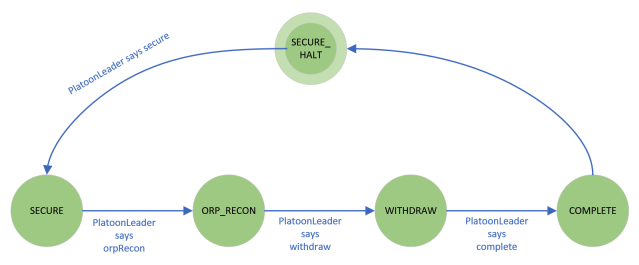
\includegraphics[width=0.85\textwidth]{../figures/ssmSecurtHaltDiagram}
\caption{\label{ssmSecurtHaltDiagram} Vertical slice: SecureHalt diagram.}
\end{figure}

ssmSecureHalt is straight forward. There is only one principal authorized to make transitions.  This is the Platoon Leader.  Everything follows sequentially.  
\clearpage

                  %%%%%%%%%%%%% Subsection ssmORPRecon %%%%%%%%%%%%%%%%%%%
\subsubsection{ssmORPRecon}\label{sssec:ssmORPRecon}
The sub-sub-sub-level ORP_RECON state is expanded into the ssmORPRecon \glsentryshort{ssm} and shown in figure \ref{ssmORPReconDiagram}.

\begin{figure}[h!]
\centering
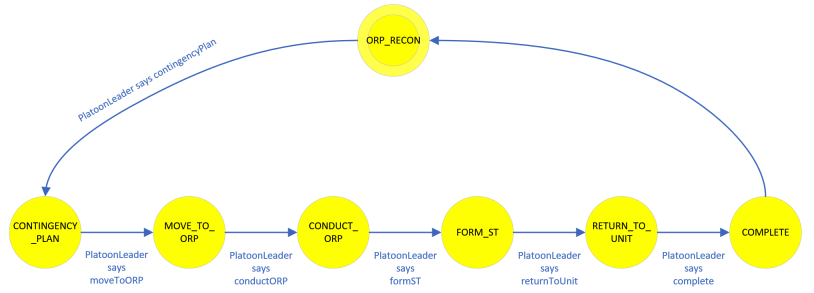
\includegraphics[width=\textwidth]{../figures/ssmORPReconDiagram}
\caption{\label{ssmORPReconDiagram} Vertical slice: ORPRecon diagram.}
\end{figure}

ssmOPRRecon is straight forward. There is only one principal authorized to make transitions.  This is the Platoon Leader.  Everything follows sequentially.  

\clearpage
                  %%%%%%%%%%%%% Subsection ssmMoveToORP4L %%%%%%%%%%%%%%%%%
\subsubsection{ssmMoveToORP4L}\label{sssec:ssmMoveToORP4L}
The 4th level MOVE_TO_ORP state is expanded into the ssmMoveToORP4L \glsentryshort{ssm} and shown in figure \ref{moveToORP4LDiagram}.  Recall that there is no module at the 5th level.  

\begin{figure}[h!]
\centering
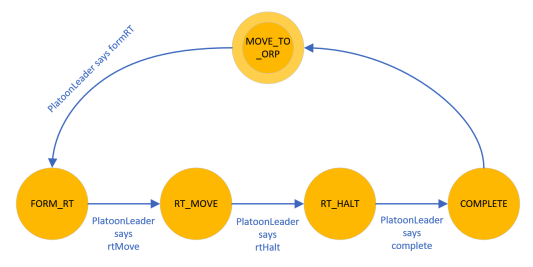
\includegraphics[width=0.85\textwidth]{../figures/moveToORP4LDiagram}
\caption{\label{moveToORP4LDiagram} Vertical slice: MoveToORP4L diagram.}
\end{figure}

ssmMoveToORP4L is straight forward. There is only one principal authorized to make transitions.  This is the Platoon Leader.  Everything follows sequentially.  
\clearpage

                  %%%%%%%%%%%%% Subsection ssmFormRT %%%%%%%%%%%%%%%%%%%%
\subsubsection{ssmFormRT}\label{sssec:ssmFormRT}
The 6th level FORM_RT state is expanded into the ssmFormRT \glsentryshort{ssm} and shown in figure \ref{moveToORP4LDiagram}.  (Recall that there is no module at the 5th level for this slice.  Also, the 8th level is not modeled.)

\begin{figure}[h!]
\centering
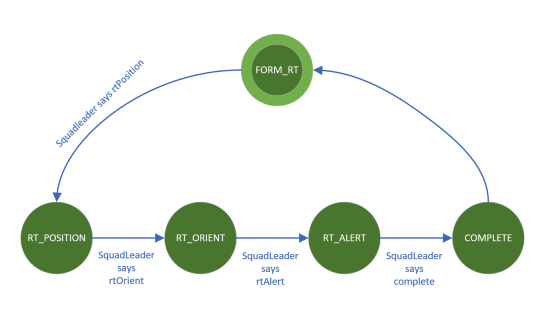
\includegraphics[width=0.85\textwidth]{../figures/ssmFormRTDiagram}
\caption{\label{ssmFormRTDiagram} Vertical slice: FormRT diagram.}
\end{figure}

ssmFormRT is straight forward. There is only one principal authorized to make transitions.  This is the Squad Leader.  Everything follows sequentially.  

\end{document}